% !TEX encoding = UTF-8 Unicode
\documentclass[a4paper]{article}
%%%%%%%%%%%%%%%%%%%%%%%%%%%%%%%%%%%%%%%%%%%%%%%%%%%%%%%%%%%%%%%%%%%
% Packages using
%%%%%%%%%%%%%%%%%%%%%%%%%%%%%%%%%%%%%%%%%%%%%%%%%%%%%%%%%%%%%%%%%%%
\ifx\pdfoutput\undefined
\usepackage[dvips]{graphicx}
\DeclareGraphicsExtensions{.eps}
\else
\usepackage[pdftex]{graphicx}
\DeclareGraphicsExtensions{.pdf,.jpg,.png,.mps}
\pdfcompresslevel=9
\fi

\usepackage{color}
\usepackage{adjustbox}
\usepackage{enumitem}
\usepackage{xparse}
\usepackage[a4paper, total={6in, 8in}]{geometry}
%\usepackage[round,authoryear]{natbib}
\usepackage[utf8]{inputenc}
\usepackage[english]{babel}
\usepackage{indentfirst}
\addtolength{\topmargin}{-20mm}
\addtolength{\textheight}{70mm}
\usepackage{amsmath} % Added to get modern math environments
\usepackage{bm}
\usepackage{amssymb,amsfonts} %Added to get math
\usepackage{amsthm} % Added to get theorems
\usepackage{natbib} % Added to get better bibliography
\usepackage{soul} %underline
\usepackage{url}
% Special hack below to break the URL!
\def\UrlBreaks{\do\.\do\@\do\\\do\/\do\!\do\_\do\|\do\;\do\>\do\]%
	\do\)\do\,\do\?\do\'\do+\do\=\do\#\do\i\do\m\do\t\do\a\do\x}%
\urlstyle{rm} %
\usepackage[bookmarks=true,bookmarksnumbered=true,hypertexnames=true,breaklinks=true,colorlinks=true]{hyperref}
\hypersetup{
	pdfauthor = {Ubadigha Chinweze},
	pdftitle = {Information Retrieval and Processing--Setup of a Full Text System Implementing Automatic Metadata Extraction and Visualization},
	pdfsubject = {Set-Up Guide},
	pdfkeywords = {Django, Nginx, Postgres, Gunicorn, centOS 7}}

% Headers and footers (must be after the document settings)
\usepackage{fancyhdr} %Custom header package
\pagestyle{fancy} %Turn on fancy headers
\renewcommand{\headrulewidth}{0.4pt} %Header line
\renewcommand{\footrulewidth}{0.4pt} %Footer line

% Select what to do with todonotes: 
% \usepackage[disable]{todonotes} % notes not showed
\usepackage[draft]{todonotes}   % notes showed


%%%%%%%%%%%%%%%%%%%%%%%%%%%%%%%%%%%%%%%%%%%%%%%%%%%%%%%%%%%%%%%%%%%

\title{Step-by-step Procedure to Set Up Django with Postgres, Nginx, and Gunicorn on CentOS 7} 
%\author{Chinweze Ubadigha} 
\date{\today} 

\makeatletter
\def\step{%
	\@ifnextchar[ \@myitem{\@noitemargtrue\@myitem[\@itemlabel]}}
\def\@myitem[#1]{\item[#1]\mbox{}\\}
\makeatother


% Custom environments
\newenvironment{Step}{%
	\begin{enumerate}[label= \textbf {Step} \arabic*,align=left, leftmargin=1.0cm]%
	}{
\end{enumerate}%
}

\newenvironment{Thing}{%
	\begin{enumerate}[label=Thing \arabic*,align=left, leftmargin=1.0cm]%
	}{
\end{enumerate}%
}

\begin{document}
\maketitle

\section*{Introduction}
 \label{introduction}
Before we begin lets review briefly Django, Postgres, Gunicorn, Nginx and also why we chose to use these in
setting up our web server.  Django is a web framework which can be created using python application. Django
offers simplified development server but for anything slightly production related a more powerful and
secure web server is required \citenum{DigitalOceaInc}. 
Django comes with default SQlite database but we will be using PostgreSQL a more powerful open source
object-relational database system instead \citenum{ThePostgreSQLGlobalDevelopmentGroup}. Thinking of security, NGINX is a free, open-source, high-performance HTTP server and reverse proxy \citenum{NGINXInc}. By reverse proxy, it enhances security and manages the web
traffic.\\ 
Gunicorn is an application server we will use to interface with our Django python applications and NGINX. Combining the features of these applications our Django web server will be security and performance enhanced. \par

\section* {Prerequisites}
\label{prerequisite}
Things you should have handy in order to complete this guide:

\begin{enumerate}
	\item CentOS 7 server.
	\item Sudo password (user should have sudo privileges).
	\item virtual environment. If you don't have any never mind, you will be guided on how to do that when the time comes.\\
\end{enumerate}

Lets get started,\\

\section* {Step by step procedure}
\begin{Step}
	\step
    \begin{minipage}[t]{\linewidth}
		\raggedright
		\adjustbox{valign=t}{%
			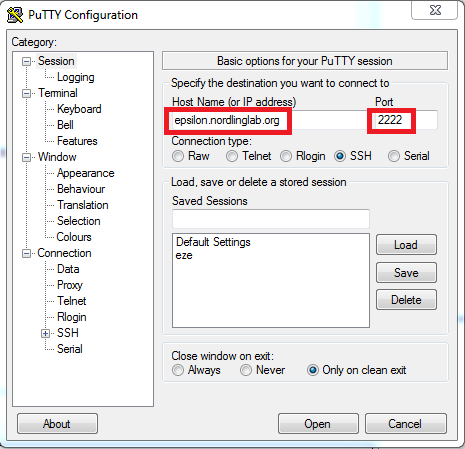
\includegraphics[width=.4\linewidth]{putty}
		}
		
		\medskip
		Login in to the server through putty using the following and as shown above.\\ %\autoref{fig:putty}:\\ \\
		Host name or IP address: \textbf{epsilon.nordlinglab.org}\\
		Port: \textbf{2222}\\
	\end{minipage}
	
%	\begin{figure}[h!]
%		\centering
%		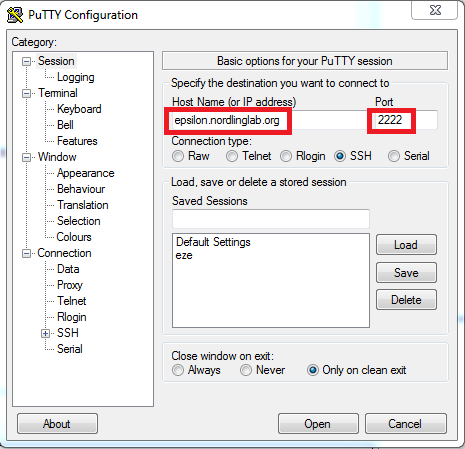
\includegraphics[scale=0.6]{putty}
%		\caption{putty login screen}
%		\label{fig:putty}
%	\end{figure}
	
	\step
	\begin{minipage}[t]{\linewidth}
		\raggedright
		\adjustbox{valign=t}{%
			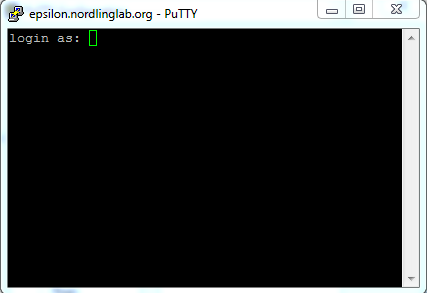
\includegraphics[width=.6\linewidth]{putty_screen}
		}
		
		\medskip
		A black screen will open as shown above. You will be prompted to key-in your \textbf{user name} followed by a \textbf{password}. Please do that.\\
	\end{minipage}		
\step
Now you've logged into the server. We will start right away to install the packages from EPEL and the
CentOS Repositories. Afterwards, we will use Python package manager \textbf{\textit{pip}} to install some
additional components.\\ Type the following in the command window to enable EPEL repository. When prompted
for the sudo password please type it.\\ \\
\textbf{\emph{sudo yum install epel-release}}\\ \\
With the new repository available, we can install all we needed in one command.
\step
Type the following into the command window:\\ \\
\textbf{\emph{sudo yum install python-pip python-devel postgresql-server postgresql-devel postgresql-contrib gcc nginx}}\\ 
\step
Configure and Start PostgreSQL. First, initialize the PostgreSQL database. We can do that by typing:\\ \\
\textbf{\emph{sudo postgresql-setup initdb}}\\
\step
Start the PostgreSQL service by typing:\\ \\
\textbf{\emph{sudo systemctl start postgresql}}\\
\step
Change the authentication method for the database to allow our Django instance user to have access using password. Type the following to edit using \textbf{nano} editor. Remember when prompted for password please type it.\\ \\
\textbf{\emph{sudo nano /var/lib/pgsql/data/pg\_hba.conf}}\\
\step
\medskip When the file opens, move to the bottom of the page and edit the file as shown below. Modify the two host lines by changing the last column (the authentication method) to \textbf{md5}. This will allow password authentication:\\
\begin{minipage}[t]{\linewidth}
	\raggedright
	\adjustbox{valign=t}{%
		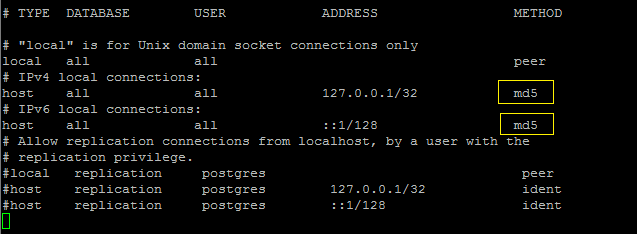
\includegraphics[width=1.0\linewidth]{post_auth}
	}\\
	
	\medskip
	When you are finished, save and close the file by clicking \textbf{ctrl C} followed by \textbf{"Y"} and then \textbf{"Enter"}. \\
\end{minipage}

\step
Restart the service and also enable the PostgreSQL so that it start automatically at boot:\\ \\
\textbf{\emph{sudo systemctl restart postgresql}}
\textbf{\emph{sudo systemctl enable postgresql}}\\
\step
It will be convenient to change to root user temporarily in order to work with postgres locally. Type\\ \\
\textbf{\emph{sudo su - postgres}}\\ \\followed by\\ \\
\textbf{\emph{psql}}\\ \\
This will be give you a PostgreSQL prompt where we can set up our requirements.\\

\step
Creat a database for our project:\\ \\
\textbf{\emph{CREATE DATABASE \textcolor{red}{myproject};}}\\ \\
Next create database user for our project:\\ \\
\textbf{\emph{CREATE USER \textcolor{red}{myprojectuser} WITH PASSWORD '\textcolor{red}{password}';}}\\ \\
Give our new user access to administer our new database:\\ \\
\textbf{\emph{GRANT ALL PRIVILEGES ON DATABASE \textcolor{red}{myproject} TO \textcolor{red}{myprojectuser};}}\\ \\
Notice all the command must end with semicolon. When you are done exit the postgreSQL promtp by typing:\\ \\
\bm{$\backslash q$}\\ \\
Now also exit the root user by typing:\\ \\
\textbf{\emph{exit}}\\

\step
We now create our python virtual environment for your Django Project. If you already have virtualenv install you skip this step, else type:\\ \\
\textbf{\emph{sudo pip install virtualenv}}\\ \\


\end{Step}
	
	
	
	
	











	%%%%%%%%%%%%%%%%%%%%%%%%%%%%%%%%%%%%%%%%%%%%%%%%%%%%%%%%%%%%%%%%%%%
	% References
	% Using Mendeley Desktop with library.bib
	%%%%%%%%%%%%%%%%%%%%%%%%%%%%%%%%%%%%%%%%%%%%%%%%%%%%%%%%%%%%%%%%%%%	
	\newpage	
	\bibliographystyle{agsm_nurl}
	\bibliography{library}	
	\clearpage 

\end{document}